\section{Auswertung}
\subsection{Bestimmung der maximalen Kraftflussdichte des Magnetfeldes}

Zunächst werden in Abbildung \ref{fig:B(z)} die aufgenommenen Daten (siehe Tabelle \ref{tab:B(z)}) der Magnetfeldstärke gegen den Ort in der Spule aufgetragen.

\begin{figure}[H]
  \centering
  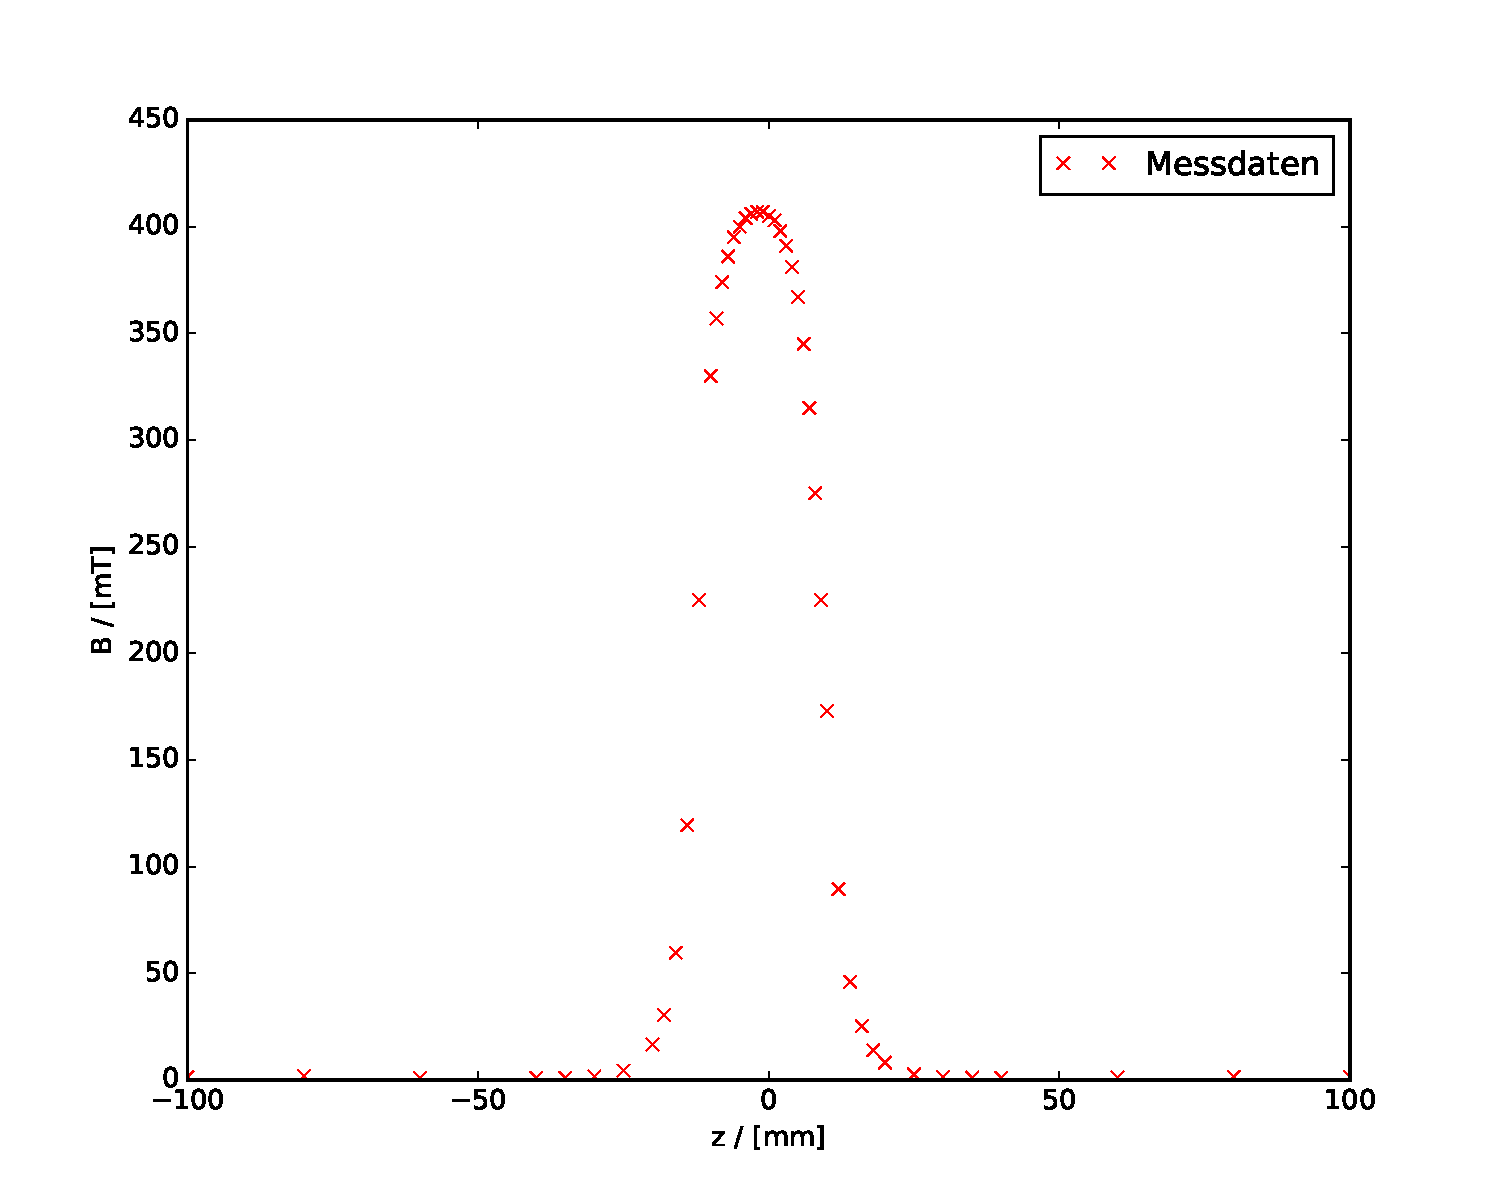
\includegraphics
  [width=\textwidth]{B-Feld.pdf}
  \caption{Kraftflussdichte des Magnetfeldes in Abhängigkeit von dem Ort der Spule}
  \label{fig:B(z)}
\end{figure}

\begin{table}[H]
  \centering
  \begin{tabular}{cc}
    \toprule
    Ort $z$ / [cm] & Magnetfeldstärke $B$ / [mT] \\
    \midrule
    -002 & 407,0 \\
    -100 & 1,300 \\
    -080 & 1,880 \\
    -060 & 1,000 \\
    -040 & 0,970 \\
    -035 & 1,100 \\
    -030 & 1,690 \\
    -025 & 4,360 \\
    -020 & 16,60 \\
    -018 & 30,50 \\
    -016 & 59,70 \\
    -014 & 119,4 \\
    -012 & 225,0 \\
    -010 & 330,0 \\
    -009 & 357,0 \\
    -008 & 374,0 \\
    -007 & 386,0 \\
    -006 & 395,0 \\
    -005 & 400,0 \\
    -004 & 404,0 \\
    -003 & 406,0 \\
    -001 & 407,0 \\
    0000 & 405,0 \\
    0001 & 403,0 \\
    0002 & 398,0 \\
    0003 & 391,0 \\
    0004 & 381,0 \\
    0005 & 367,0 \\
    0006 & 345,0 \\
    0007 & 315,0 \\
    0008 & 275,0 \\
    0009 & 225,0 \\
    0010 & 173,0 \\
    0012 & 89,50 \\
    0014 & 46,10 \\
    0016 & 25,20 \\
    0018 & 14,00 \\
    0020 & 8,170 \\
    0025 & 2,630 \\
    0030 & 1,390 \\
    0035 & 1,120 \\
    0040 & 1,080 \\
    0060 & 1,140 \\
    0080 & 1,460 \\
    0100 & 1,340 \\
    \bottomrule
  \end{tabular}
  \caption{Magnetfeldstärke in Anhängigkeit von dem Ort}
  \label{tab:B(z)}
\end{table}

Die maximale Kraftflussdichte des Magnetfeldes entspricht der Magnetfeldstärke am Ort der Probe.
Somit ergibt sich die Kraftflussdichte von
\begin{align}
  B_0 = 407\si{\milli\tesla}.
  \label{b}
\end{align}

\subsection{Bestimmung der effektiven Masse}
In Tabelle \ref{tab:proben} werden die drei verwendeten Proben mit einigen Daten aufgelistet.

\begin{table}[H]
  \centering
  \begin{tabular}{ccc}
    \toprule
    Probe & Dotierung / [$\frac{1}{\text{cm}^3}$] & Dicke $L$ / [mm] \\
    \midrule
    1. GaAs & $1.2\cdot10^{8}$ & 1,36 \\
    2. GaAs & $2.8\cdot10^{18}$ & 1,296 \\
    3. GaAs & - & 5,11 \\
    \bottomrule
  \end{tabular}
  \caption{Dotierung und Dicke der verwendeten GaAs-Proben}
  \label{tab:proben}
\end{table}

Die Rotationswinkel der Polarisationsebenen werden mit Hilfe der Formel
\begin{equation}
  \theta = \sqrt{\left(\frac{1}{2}(\theta_1 - \theta_2)\right)^2}
  \label{eqn:thetadiff}
\end{equation}
berechnet.
Die zu den Proben entsprechenden Winkel werden in Tabelle \ref{tab:winkel} aufgelistet.

\begin{table}

  \centering
\begin{tabular}{c|c|c|c|c|c|c}

  \toprule
  & \multicolumn{3}{|c|}{Winkel $\theta_{1,2,3}$} & \multicolumn{3}{|c|}{Normierter Winkel $({\frac{\theta}{L}})_{1,2,3}$ / [$\frac{1}{\text{mm}}$]} \\
  Wellenlänge $\lambda$ / [$\si{\micro}$m] & Probe 1 & Probe 2 & Probe 3 & Probe 1 & Probe 2 & Probe 3 \\

  \midrule
  1.06 & 9.695° & 11.455° & 12.600° & 7.129° &  8.839°  & 2.466°  \\

  1.29 & 0.445° & 19.010° &  7.390° & 1.390° &  4.726°  & 5.682°  \\
  1.72 & 1.625° & 28.125° & 21.705° & 1.779° &  4.136°  & 0.442° \\
  1.96 & 2.420° &  5.360° &  2.260° & 1.195° & 21.701°  & 4.248°  \\
  2.16 & 1.890° &  6.125° & 29.035° & 4.051° &  7.299°  & 0.366° \\

  2.34 & 3.400° & 54.725° &  1.840° & 7.088° &  3.457°  & 0.141° \\
  2.51 & 9.640° &  4.480° &  0.720° & 2.500° & 42.226°  & 0.360° \\
  2.65 & 5.510° &  9.460° &  1.870° & 0.327° & 14.668°  & 1.446°  \\
  \bottomrule
\end{tabular}
\caption{Rotationswinkel der Polarisationsebenen der verwendeten Proben bei verschiedenen Wellenlängen.}

\label{tab:winkel}
\end{table}



Im Diagramm \ref{fig:0(y)} werden übersichtshalber die normierten Rotationswinkel gegenüber der Wellenlängen aufgetragen.

\begin{figure}[H]
  \centering
  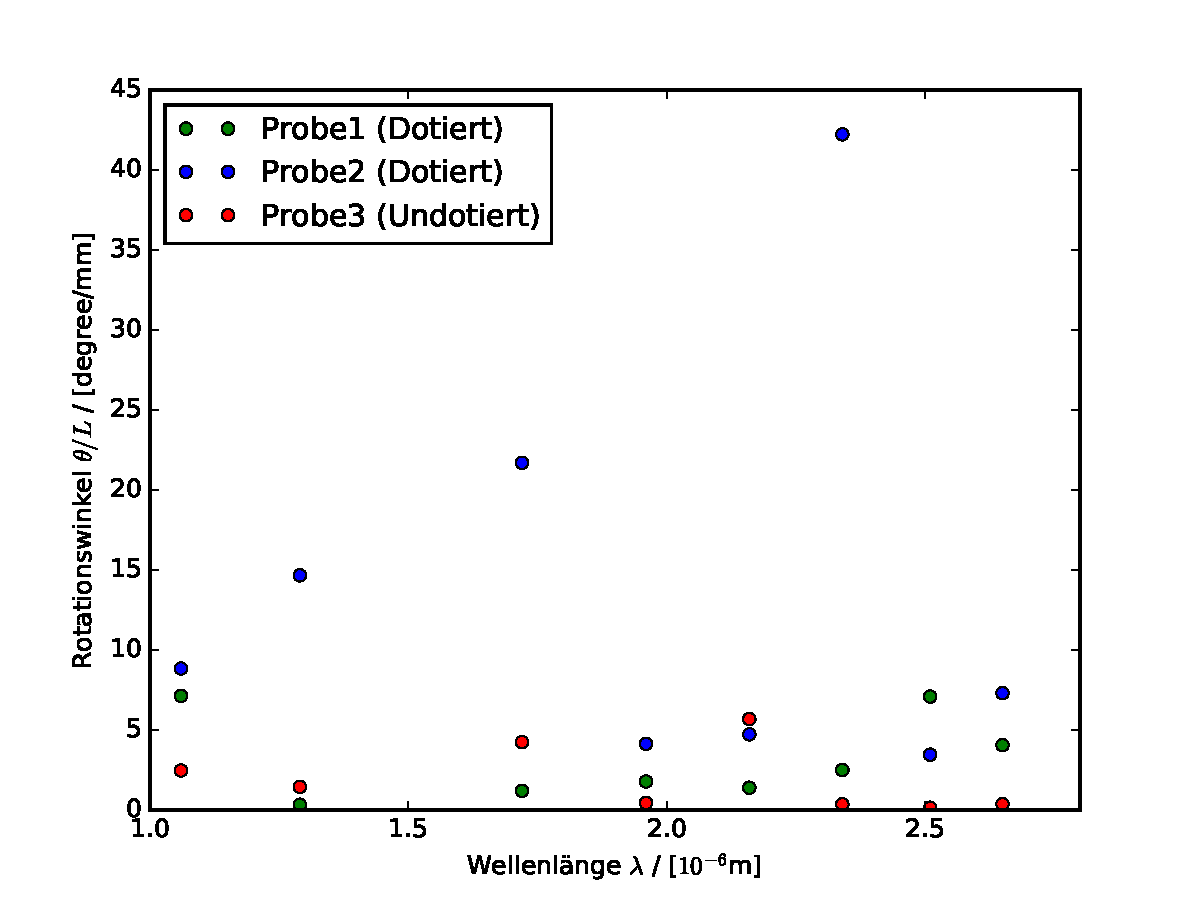
\includegraphics
  [width=\textwidth]{winkelplot.pdf}
  \caption{Rotationswinkel in Abhängigkeit von der Wellenlänge der Proben im Vergleich}
  \label{fig:0(y)}
\end{figure}

Als nächstes wird der Betrag der Differenz der Faraday-Rotation zwischen dotierter und reiner Probe gebildet.
Dies kann Tabelle \ref{tab:difftab} entnommen werden.

\begin{table}

  \centering
\begin{tabular}{c|c|c}

  \toprule
Wellenlänge $\lambda$ / [$\si{\micro}$m] & $|\frac{\theta_1}{L_1}-\frac{\theta_3}{L_3}$| & |$\frac{\theta_2}{L_2}-\frac{\theta_3}{L_3}$| \\

\midrule
1,06 & 4,663 &  6,373 \\

1,29 & 4,292 &  0,956 \\

1,72 & \textcolor{red}{1,337} &  3,694 \\

1,96 & 3,053 & 17,453 \\

2,16 & 3,685 &  6,933 \\

2,34 & \textcolor{red}{6,947} &  3,316 \\

2,51 & 2,14  & \textcolor{red}{41,866} \\

2,65 & 1,119 & 13,222 \\
\bottomrule

\end{tabular}
\caption{Beträge der Differenzen der Faraday-Rotationen zwischen dotierter und reiner Probe}

\label{tab:difftab}
\end{table}



Die Formel
\begin{equation}
  \frac{\theta}{L} = \frac{e_0^3}{8\pi^2\epsilon_0c^3m^2}\frac{NB}{n}\cdot\lambda^2
\end{equation}
hat die Form
\begin{equation}
  \frac{\theta}{L} = \alpha\cdot x + \beta
\end{equation}
mit $x=\lambda^2$.
Mit einer Ausgleichsrechnung lässt sich der experimentelle Faktor $\alpha$ bestimmen.

Den Abbildungen \ref{fig:winkeldiff1} und \ref{fig:winkeldiff2} können die Differenzen zwischen dotierter und reiner Probe in Abhängigkeit von der Wellenlänge zum Quadrat und die entsprechende Ausgleichsgerade entnommen werden.
Die rot markierten Werte aus Tabelle \ref{tab:difftab} werden aufgrund ihrer hohen Abweichung nicht berücksichtigt.

\begin{figure}[H]
  \centering
  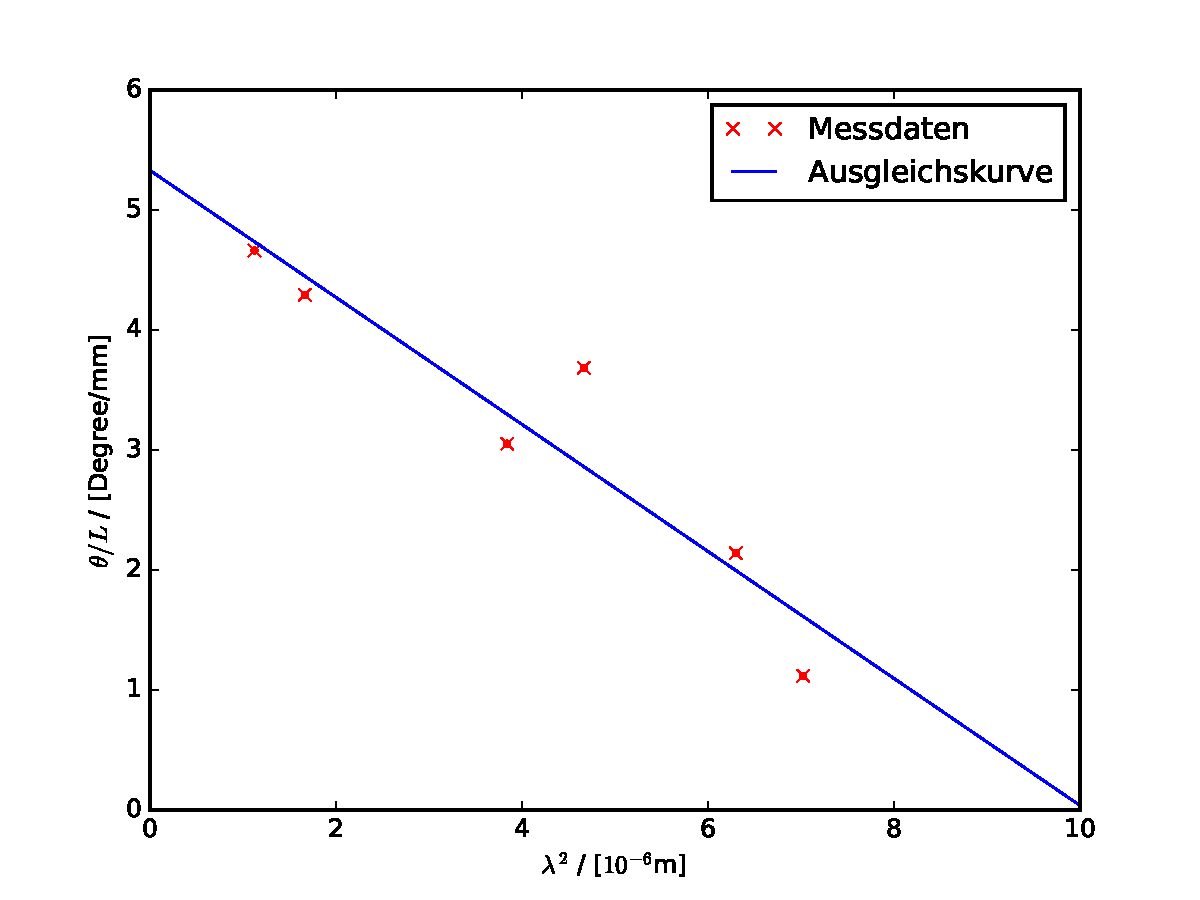
\includegraphics
  [width=\textwidth]{winkeldiffplot1.pdf}
  \caption{Ausgleichskurve für die Differenz der Faradayrotation zwischen dotierter und reiner Probe in Abhängigkeit von der Wellenlänge zum Quadrat der Probe 1.}
  \label{fig:winkeldiff1}
\end{figure}
Die mit Python berechneten Parameter sind
\begin{gather*}
  \alpha_1 = 0,53 \pm 0,10 \\
  \beta_1 = 5,3 \pm 0,5
\end{gather*}

\begin{figure}[H]
\centering
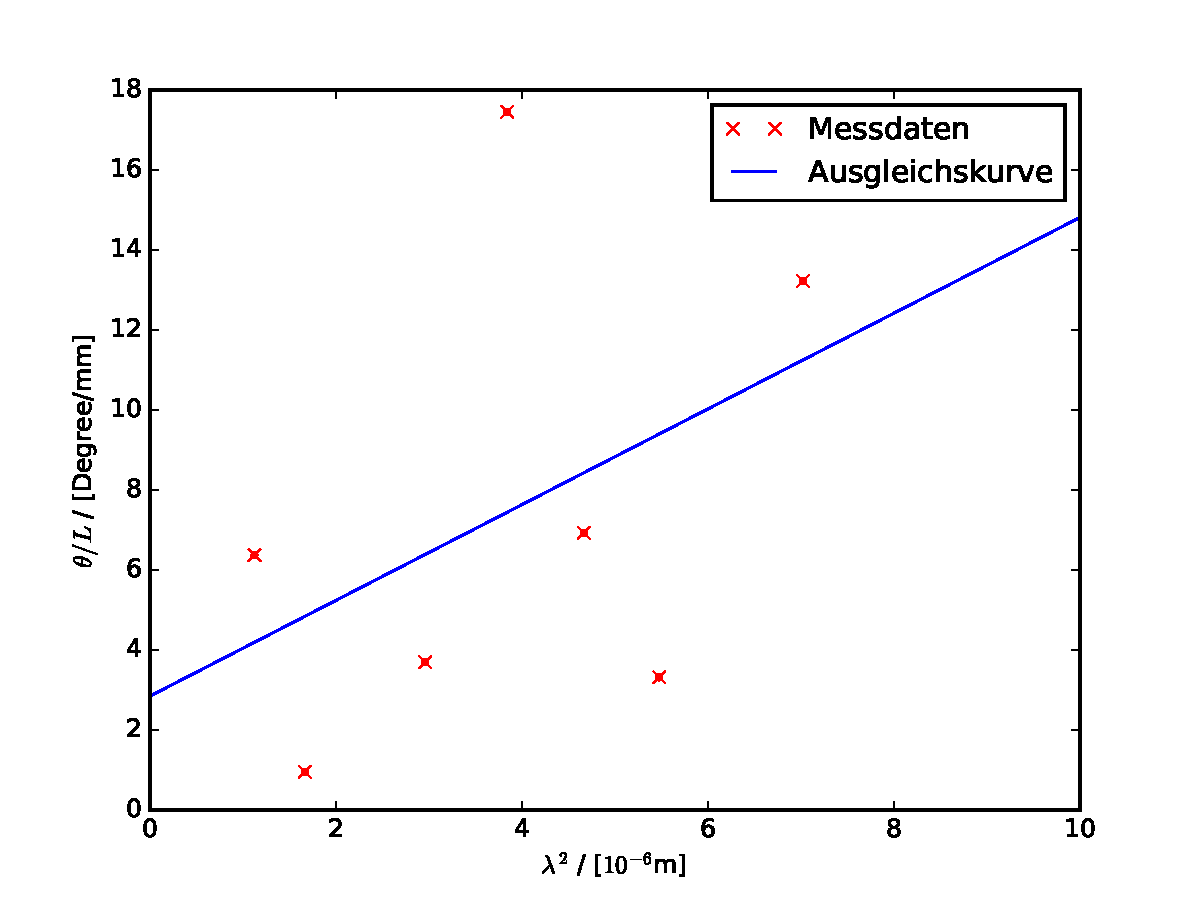
\includegraphics
[width=\textwidth]{winkeldiffplot2.pdf}
\caption{Ausgleichskurve für die Differenz der Faradayrotation zwischen dotierter und reiner Probe in Abhängigkeit von der Wellenlänge zum Quadrat der Probe 2.}
\label{fig:winkeldiff2}
\end{figure}
Die mit Python berechneten Parameter sind
\begin{gather*}
    \alpha_2 = 1,2 \pm 1,1 \\
    \beta_2 = 2,8 \pm 5
\end{gather*}

Die effektive Masse lässt sich nun bestimmen, indem
\begin{equation}
  \alpha_{1,2} = \frac{e_0^3N_{1,2}B}{8\pi^2\epsilon_0c^3m^2n}
  \label{eqn:vorfaktor}
\end{equation}
nach $m$ umgestellt wird.
Es ergibt sich die Formel
\begin{equation}
  m_{1,2}^* = \sqrt{\frac{e_0^3N_{1,2}B}{8\pi^2\epsilon_0c^3n\alpha_{1,2}}}
  \label{eqn:m}
\end{equation}
für die effektive Masse.

In der folgenden Tabelle \ref{tab:var} können die nötigen Variablen und Konstanten für die Berechnung von \eqref{eqn:m} entnommen werden.
\begin{table}[H]
  \centering
  \begin{tabular}{ccccc}
    \toprule
    Bezeichnung & Formelzeichen & Wert & Einheit & Quelle \\
    \midrule
    Magnetische Flussdichte    & $B$          & $407\cdot10^{-3}$    & T                           & \eqref{b} \\
    Elementarladung            & $e_0$        & $1,602\cdot10^{-19}$ & C                           & \cite{pdg} \\
    Influenzkonstante          & $\epsilon_0$ & $8,854\cdot10^{-12}$ & $\sfrac{\text{F}}{\text{m}}$ & \cite{pdg} \\
    Vakuumlichtgeschwindigkeit & $c$          & $2,9979\cdot10^{8}$  & $\sfrac{\text{m}}{\text{s}}$               & \cite{pdg} \\
    Dotierung der Probe 1      & $N_1$        & $1,2\cdot10^{8}$     & $\sfrac{1}{\text{cm}^3}$     & \ref{tab:proben} \\
    Dotierung der Probe 2      & $N_2$        & $2,8\cdot10^{18}$    & $\sfrac{1}{\text{cm}^3}$     & \ref{tab:proben} \\
    Brechungsindex von GaAs    & $n$          & $3,57$               & -                           & \cite{cb} \\
    Elektronenmasse            & $m_e$        & $9,109\cdot10^{-31}$ & kg                          & \cite{pdg} \\
    \bottomrule
  \end{tabular}
  \caption{Einige Variablen und Konstanten}
  \label{tab:var}
\end{table}

Unter Berücksichtigung der Gaußschen Fehlerfortpflanzung ergeben sich
\begin{gather*}
  m_1^* = (2,4 \pm 0,3)\cdot10^{-33}\text{kg} = (0,0026 \pm 0,0003)m_e \\
  m_2^* = (2,4 \pm 1,1)\cdot10^{-28}\text{kg} = (260 \pm 130)m_e
\end{gather*}

Der Literaturwert der effektiven Masse des Elektrons im tiefsten Minimum des Leitungsbandes \cite{ru} beträgt
\begin{equation*}
  m_{\Gamma} = 0.063 m_e
\end{equation*}
